This chapter introduces the basics of quantum computing and reinforcement learning that form the backdrop of the work in the remainder of the thesis.

We start with a brief introduction of the quantum computation model and its mathematical and geometric formalism and introduce the circuit model of computation. 

Next, we discuss Quantum Algorithms, starting with pure quantum algorithms like Grover's, Shor's, and Hamiltonian simulation and move on to Variational Methods like QAOA (Quantum Approximate Optimization Algorithm) and VQE (Variational Quantum Eigensolver). The compilation and visualization of these algorithms form the basis of the work presented in this thesis. Both our algorithms have been tested extensively on some subset of these circuits. There are a small number of such subroutines that have currently been discovered in quantum algorithmic theory, and these subroutines are often and repeatedly used, motivating the value of using machine learning methods which can exploit recurring patterns to perform quantum circuit transformations as close to optimally as possible (Qubit routing results on these algorithmic benchmarks as setup by IBM are listed in \ref{ch:appendix-qroute}). The QAOA algorithm for max-cut is also our test-bed for analyzing and visualizing the learning properties of these variational circuits.

Finally, we move to a didactic introduction to reinforcement learning by talking about the different learning frameworks in the field like Value-based, Policy-based, etc. We discuss the algorithmic details of those methods that are relevant to our work, like Deep-Q-learning, Policy Gradients, Actor-Critic, and Monte Carlo Tree Search.

\section{Quantum Computation}


\subsection{Qubits and Quantum Computation Model}

Quantum Computers store information as quantum bits, or qubits. These qubits evolve through the application of unitary operators, also called gates. The gate model of quantum computation is akin to that on classical computers; the following is a diagrammatic illustration of the same:

\begin{figure}[ht]
    \centering
    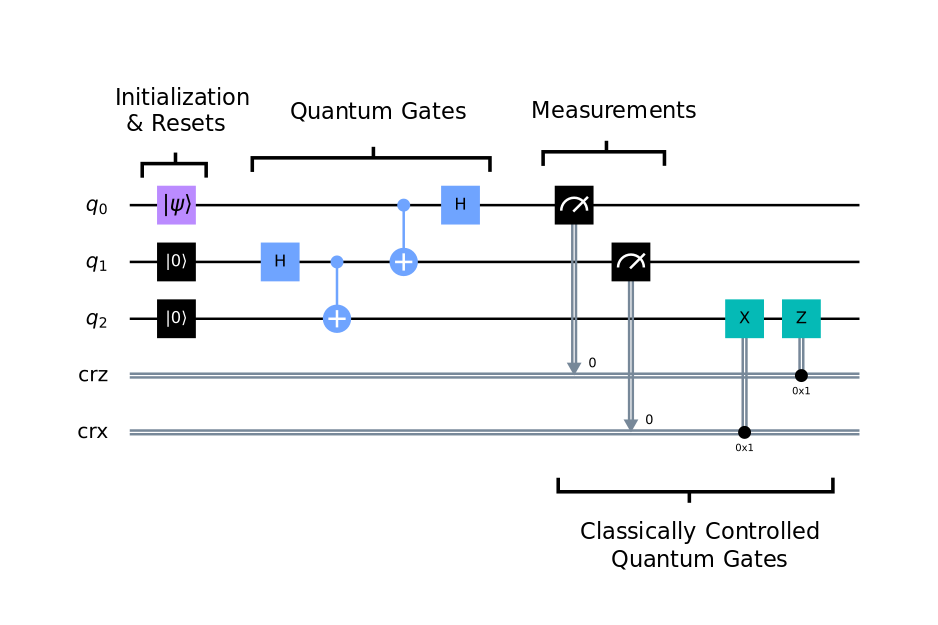
\includegraphics[width=0.8\linewidth]{figures/quantum/quantum_circuit_example.png}
    \caption[Typical Quantum Circuit]{The image shows the parts of a typical quantum circuit, with 3 qubits represented by the wires and a set of gates applied to them, followed by measurement of those qubits.}
    \label{fig:quantum-circuit-example}
\end{figure}


A classical bit can be either 0 or 1. However, a qubit can live in any state inbetween 0 or 1, which is understood as being in a weighted superposition of the 0 and 1 states. So the state of a qubit 
\begin{equation}
    \ket{\psi} = \alpha \ket{0} + \beta \ket{1} = \begin{bmatrix}\alpha \\ \beta\end{bmatrix} \;\;\text{such that }|\alpha|^2 + |\beta|^2 = 1 \text{ and } \alpha, \beta \in \mathbb{C}
\end{equation}
where the normalization of probabilities forces. However this state of the qubit is not accessible to us, and we can only measure the qubit probabilistically, with probability of being $\ket{0}$ being $|\alpha|^2$ and that of $\ket{1}$ being $\beta^2$.

Each qubit, in addition to the superposition it is in, also has a phase term, which is represented on the Bloch-sphere \ref{fig:bloch-sphere} on the $\hat{x}-\hat{y}$ plane. The phase does not affect the immediate measurement of the qubit but can affect the resultant phase and superposition when some unitary operation is applied to the qubit.

\begin{figure}[ht]
    \centering
    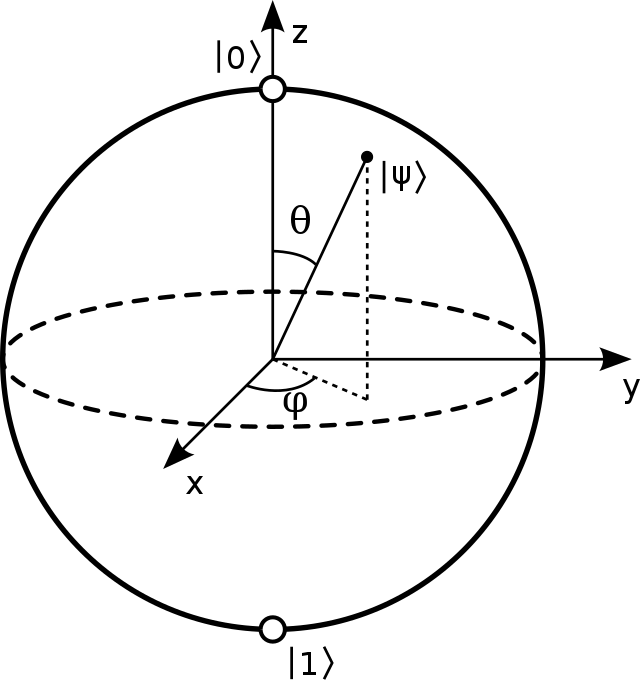
\includegraphics[width=0.4\linewidth]{figures/quantum/bloch_sphere.png}
    \caption[Block Sphere representation of Quantum States]{Bloch Sphere represents the state of a qubit $\ket{\psi}$. The pure states $\ket{0}$ and $\ket{1}$ are the vectors along the z-axis on the opposite poles. The angle along the x-y plane represents the phase of the qubits.}
    \label{fig:bloch-sphere}
\end{figure}


\subsection{Unitaries, Gates, and Entanglement}
\label{sec:background-unitary-gate-entanglement}

The state of a system of qubits can be modified by gates. The  gates that can executed on a quantum computer are those that apply norm-preserving linear transforms on the state vector.
\begin{equation}\label{eqn:gates-transforming-qubits}
    \ket{\psi_1^\prime \otimes \psi_2^\prime \otimes \ldots \otimes \psi_n^\prime} = U_{2^n \times 2^n} \ket{\psi_1 \otimes \psi_2 \otimes \ldots \otimes \psi_n}
\end{equation}
When we transform the state as $\ket{\psi} \rightarrow U \ket{\psi}$, the norm of the state transforms as $\braket{\psi | \psi} \rightarrow \braket{\psi U^\dagger \vert U \psi}$. To ensure that norm is preserved, we need the $U^\dagger U = \mathbb{I}$, so all gates on quantum computers must be unitaries.

\begin{figure}[!ht]
    \centering
    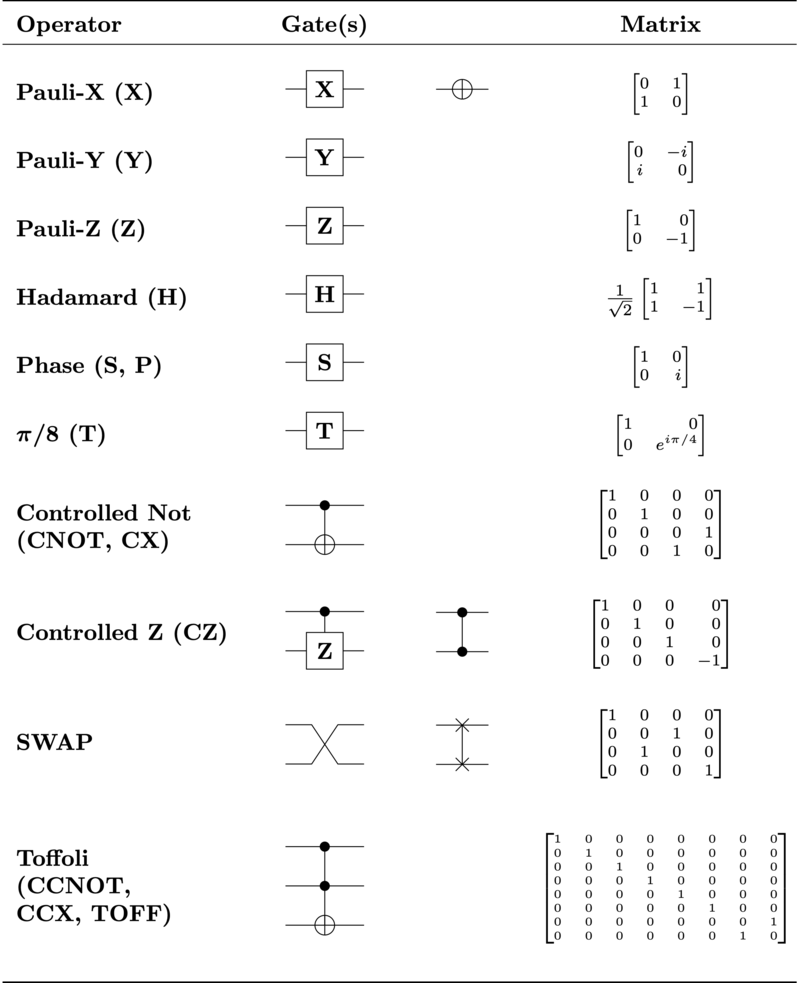
\includegraphics[width=0.6\linewidth]{figures/quantum/quantum_logic_gates.png}
    \caption[List of Logic Gates]{Popular logic gates along with their in-circuit representations and corresponding unitary matrices. $X$, $Y$, $X$, $H$, $S$, $P$ and $T$ are all single qubit gates. $X$ is a $180^o$ rotation of the bloch sphere around the $X$ axis, same with $Y$ and $Z$. $R_x(\theta) = e^{-i X \theta / 2}$ is a rotation of $\theta$ angle around the X-axis, same with the other axes. $CX$ is a controlled form of the $X$ gate, where one qubit participating in the operation is the controller, and if it's in the $\ket{1}$ state then $X$ gate will be applied on the qubit, and not if it was in the $\ket{0}$ state. Such gates result in the two qubits becoming entangled, other controlled gates are $CNOT$ (controlled version of $Z$), $CR_x(\theta)$ (Controlled version of rotation along $X$), etc. \cite{book-nielsen-chuang}}
    \label{fig:quantum-unitary-gates}
\end{figure}

Some multi-qubit gates introduce a property called Entanglement. Examples of such gates are CNOT, CZ, etc. Once two qubits are "entangled" through some such operation like CNOT, their state cannot be written as a product of the individual states of the qubits; they are now linked in a way that the probability distribution of collapsing either state along the measurement axis is not factorizable. 

The state of an entangled system of $n$-qubits can be represented by a unit-norm state-vector in $\mathbb{C}^{2^n}$. This is because each of the bit-vectors of n-bits which can be an outcome of measurement need to have their probabilities and phases represented. A linear transform on such a system is therefore defined by a matrix of shape $2^n \times 2^n$, as mentioned in equation \ref{eqn:gates-transforming-qubits}.

\subsection{Density Matrices and Noise}

State preparation on a quantum computer is subject to noise. Therefore there often exists some uncertainty in the state of qubits on actual physical hardware. This uncertainty can be modeled as a classical probability distribution over the different quantum states that might have been prepared. Such a state is called a mixed state, as opposed to a pure state. Mixed states can be represented using Density matrices $\rho$, which are 2-D matrices with $2^n \times 2^n$ elements for $n$ qubits.
\begin{equation}
    \rho = \sum_{i} p_i \ket{x_i} \bra{x_i}
\end{equation}

Much like unitary operations on state vectors (\ref{sec:background-unitary-gate-entanglement}), the application of unitaries on density matrices can be represented through simple matrix multiplication:
\begin{equation}
    \mathcal{O} (\rho) = \sum_i p_i \mathcal{O}(\ket{x_i}) \mathcal{O}(\bra{x_i}) = \sum_i p_i U \ket{x_i} \bra{x_i} U^\dagger = U \rho U^\dagger
\end{equation}


\section{Quantum Algorithms}
\label{sec:quantum-algorithms}

\subsection{Purely Quantum Algorithms}

Superposition and Entanglement together provide quantum computers with natural parallel processing power. While full access to this parallelism gets bottlenecked at the measurement layer since we can sample only one of the many states in weighted superposition, it is conceivable that for many an algorithm, this parallelism can result in a processing speed-up. A near-term goal with Quantum Computers is to achieve quantum supremacy, which is to solve a problem (possibly one of no practical use) that no classical computer can solve in a feasible amount of time. \cite{quantum-complexity-survey}

The algorithms developed for quantum computation till date can be categorized into just 3 classes \cite{quantum-algo-shor-3-classes}, listed below:
\begin{itemize}
    \item Grover Like (Amplitude Amplification class of algorithms).
    \item Shor Like (Using Quantum Phase Estimation and Quantum Fourier Transform)
    \item Hamiltonian Simulation 
\end{itemize}
All algorithms in each class share the subroutines which are the primary cause of the quantum speedup. Below we describe these three classes of algorithms in some detail.

\subsubsection{Grover's Search}

Grover's search is an algorithm to search for some target element or set of elements in an unordered list of size $n$ in $\sqrt{n}$ time proposed by Grover in 1996 \cite{grover-search-original}.

\paragraph*{The Problem}: Grover attacks the problem of unstructured search, where we have a list of $n$ elements in any permutation, and we have an oracle that marks each of these elements $1$ if it is one of the results of the search procedure we wish to find, or as $0$ if it is not one of those elements. The oracle only returns a value of $1$ for some $m$ of those elements, where $m << n$.

\paragraph*{Overview of the Algorithm}: Following is a brief explanation of how Grover's Algorithm operates:

\begin{enumerate}
    \item \textbf{Preparing the initial superposition of bitstrings:} The initial state should be the superposition of all elements in our search domain. Since these are the indices of the elements we are searching over, we can take this to be an equal superposition of all basis states, constructed by applying the hadamard gate over all qubits.
    \begin{equation}
        \ket{x} = \ket{s} = \frac{1}{\sqrt{n}} \sum_{i=1}^{n} \ket{b_i}
    \end{equation}

    \item \textbf{Application of a phase-kickback oracle:} For any input state $\ket{x}$, if it is a valid solution (i.e. $f(x) = 1$), then the oracle applies to that bitstring a negative phase factor. If $\ket{x}$ is not a basis state but rather is a superposition of states, then the oracle operates on each basis component of the state independently as shown in equation. \ref{eqn:grover-oracle}
    \begin{equation}\label{eqn:grover-oracle}
        \mathcal{O} \big(\ket{x} \big) = \mathcal{O}\bigg(\sum_i w_i(x) \ket{b_i} \bigg) = \sum_i w_i(x) \begin{cases}
            -\ket{b_i} & \text{if } f(b_i) = 1 \\
            \ket{b_i} & \text{if } f(b_i) = 0
        \end{cases}
    \end{equation}
    
    \item \textbf{Performing a reflection around the average amplitude:} Following the application of the oracle, we can apply a reflection around the mean amplitude of the superposition of all solutions via an application of the Diffuser operator.
    \begin{equation}
        \mathcal{D} \big(\ket{x} \big) = \big( 2 \ket{s}\bra{s} - 1 \big) \ket{x}
    \end{equation}
    Given that there are small number of solutions 
    \item \textbf{Repeat 2 steps above and measure the final state:} We iteratively apply the oracle and the diffuser circuit to take the present superposition closer and closer to the goal state. Measurement of this state along the computational basis gives us a bitstring, which with some constant probability is the solution $x$ such that $f(x) = 1$.
\end{enumerate}

\paragraph*{Ampliture Amplification algorithms}: The algorithmic structure proposed by Grover can be extended to solve other problems, the notion being that a quantum circuit that finds an algorithm with probability $p$ needs to be run only $O(1/\sqrt{p})$ times and not $O(1/p)$ times \cite{quantum-amplitude-amplification-algorithms}.

\subsubsection{Shor's Algorithm}

Shor's Algorithm is used to perform factorization of an integer product of two large prime numbers \cite{shor-quantum-algorithm-explaination}.

\paragraph*{The problem}: Given an integer that is known to be the product of two large prime numbers, we have to factor the number back into the composing integers.

\paragraph*{Overview of the Algorithm}: Following is a brief explanation of how Shor's Algorithm works:

\begin{enumerate}
    \item \textbf{Preparing the Unitary}: We need to model a unitary operator which performs modular multiplication by some constant $a$.
    \begin{equation}
        U \ket{y} = \ket{ay \;\text{mod}\; N}
    \end{equation}
    The n-qubit states for our quantum system are being represented as $\ket{0}, \ket{1}, \cdots \ket{N - 1}$, on the qubits they are being represented as the bitstrings corresponding to those numbers.
    \item \textbf{Period Finding to Phase Estimation}: Generate a linear combination of states which is an eigenstate of the unitary operator. The states in the linear combination will form an r-element subgroup, and the phase terms multiplied to each state will be the r-th roots of unity.
    \begin{equation}
        \ket{u_s} = \frac{1}{\sqrt{r}} \sum_{k=0}^{r-1} e^{-\frac{2\pi i s k}{r}} \ket{a^k \mod N}
    \end{equation}
    \begin{equation}
        U \ket{u_s} = e^{\frac{2 \pi i s}{r}} \ket{u_s}
    \end{equation}
    \item \textbf{Period Finding to Factorization}: We compute the phase $\frac{s}{r}$ from the process above. Using this, we can generate a fractional approximation to the phase and estimate the value of r. We know that
    \begin{equation}
        a^r \mod N = 1
    \end{equation}
    With high probability, r is even; if it's not then we will repeat this process with a new a. Given the above, we can guess a factor of $N$ as $a^{r/2} - 1$ or $a^{r/2} + 1$.
    \begin{equation}
        (a^{r/2} - 1) (a^{r/2} + 1) \mod N = 0
    \end{equation}
    Having ensured initially that $a$ is not a factor of $N$, we have found a high-probability guess for the factors being one of these two numbers. We repeat this process until this guess turns out to be correct.
\end{enumerate}

\paragraph*{Other Comments}: Shor's Algorithm provides an exponential advantage over any known classical algorithm, it demands too many qubits, and that fault tolerance be implemented; these are at present infeasible. An entire class of Quantum Algorithms takes inspiration from this use of period finding using the Quantum Phase Estimation process, and one prominent example is the HHL algorithm \cite{quantum-algo-hhl} for solving linear systems.

\subsubsection{Hamiltonian Simulation}

Nature is hard to simulate on a classical computer. Writing down quantum wavefunctions and updating them is computationally very expensive. As Richard Feynman said: \textit{"Nature is not classical, dammit, and if you want to make a simulation of nature, you'd better make it quantum mechanical, and by golly, it's a wonderful problem, because it doesn't look so easy." } \cite{feynman-quantum-simulating-physics}.

The most natural solution is to use the quantum systems to emulate other quantum systems and perform these computations. It seems intuitive that quantum computers are efficient at doing quantum simulations; all that needs to be done is that the state of an arbitrary system needs to be mapped onto that of ours.

There are many ways of performing Hamiltonian simulation on general-purpose gate-based quantum computers. Some of those methods are listed below:
\begin{itemize}
    \item Using Trotterization \cite{method-suzuki-trotter-decomposition}: Given a hamiltonian which can be represented as a linear combination of local Hamiltonians, $H = A + B + C$, the trotter decomposition of Unitary corresponding to the Hamiltonian can be approximated by
    \begin{equation}
        U = e^{-i H t} = (e^{-i A t / r} e^{-i B t / r} e^{-i C t / r})^r
    \end{equation}
    For larger values of $r$ this results in a pretty accurate simulation.
    \item Using Taylor Expansion of Hamiltonian \cite{hamiltonian-sim-methods-taylor}: The Hamiltonian can be expanded out as a sum of unitaries, and then the corresponding unitary can be taylor-series expanded out as a linear combination of the unitaries corresponding to terms of the Taylor expansion.
    \begin{equation}
        U = e^{-i H t} = \sum_{n=0}^{\infty} \frac{(-i H t)^n}{n!}
    \end{equation}
    \item Using Quantum Walks \cite{hamiltonian-sim-methods-qwalks}: Quantum walks can be constructed corresponding to the Hamiltonian such that the spectrum of the graph on which the walk is constructed is such that its eigenvalues correspond to the ground state of the target Hamiltonian.
    \item Using Quantum Signal Processing \cite{hamiltonian-sim-methods-qsp-1,hamiltonian-sim-methods-qsp-2}: The QSP algorithm transduces eigenvalues of the Hamiltonian into an ancilla, then transforms the eigenvalues with single-qubit rotations, and finally projects it back to the ancilla.
\end{itemize}


\subsection{Variational Circuits}
\label{sec:variational-circuits}

In the previous section, we have discussed purely quantum algorithms, which possess an advantage over their present classical competitors but need fault-tolerant quantum computers with many qubits to be executed.

In this section, we look at a few hybrid quantum-classical optimization algorithms, called variational quantum algorithms. 

Each optimization problem is solved over a parameter space and attempts to maximize some metric which we call the loss. For a quantum circuit, we can visualize the loss function as some hamiltonian for which we are trying to find the lowest energy state, i.e., the ground eigenstate. Some parametrized circuit generates this ground eigenstate, and a classical optimizer is responsible for finding as low an energy state as possible.

\subsubsection{Quantum Approximate Optimization Algorithm}
\label{sec:variational-circuits-qaoa}

\begin{figure}[ht]
    \centering
    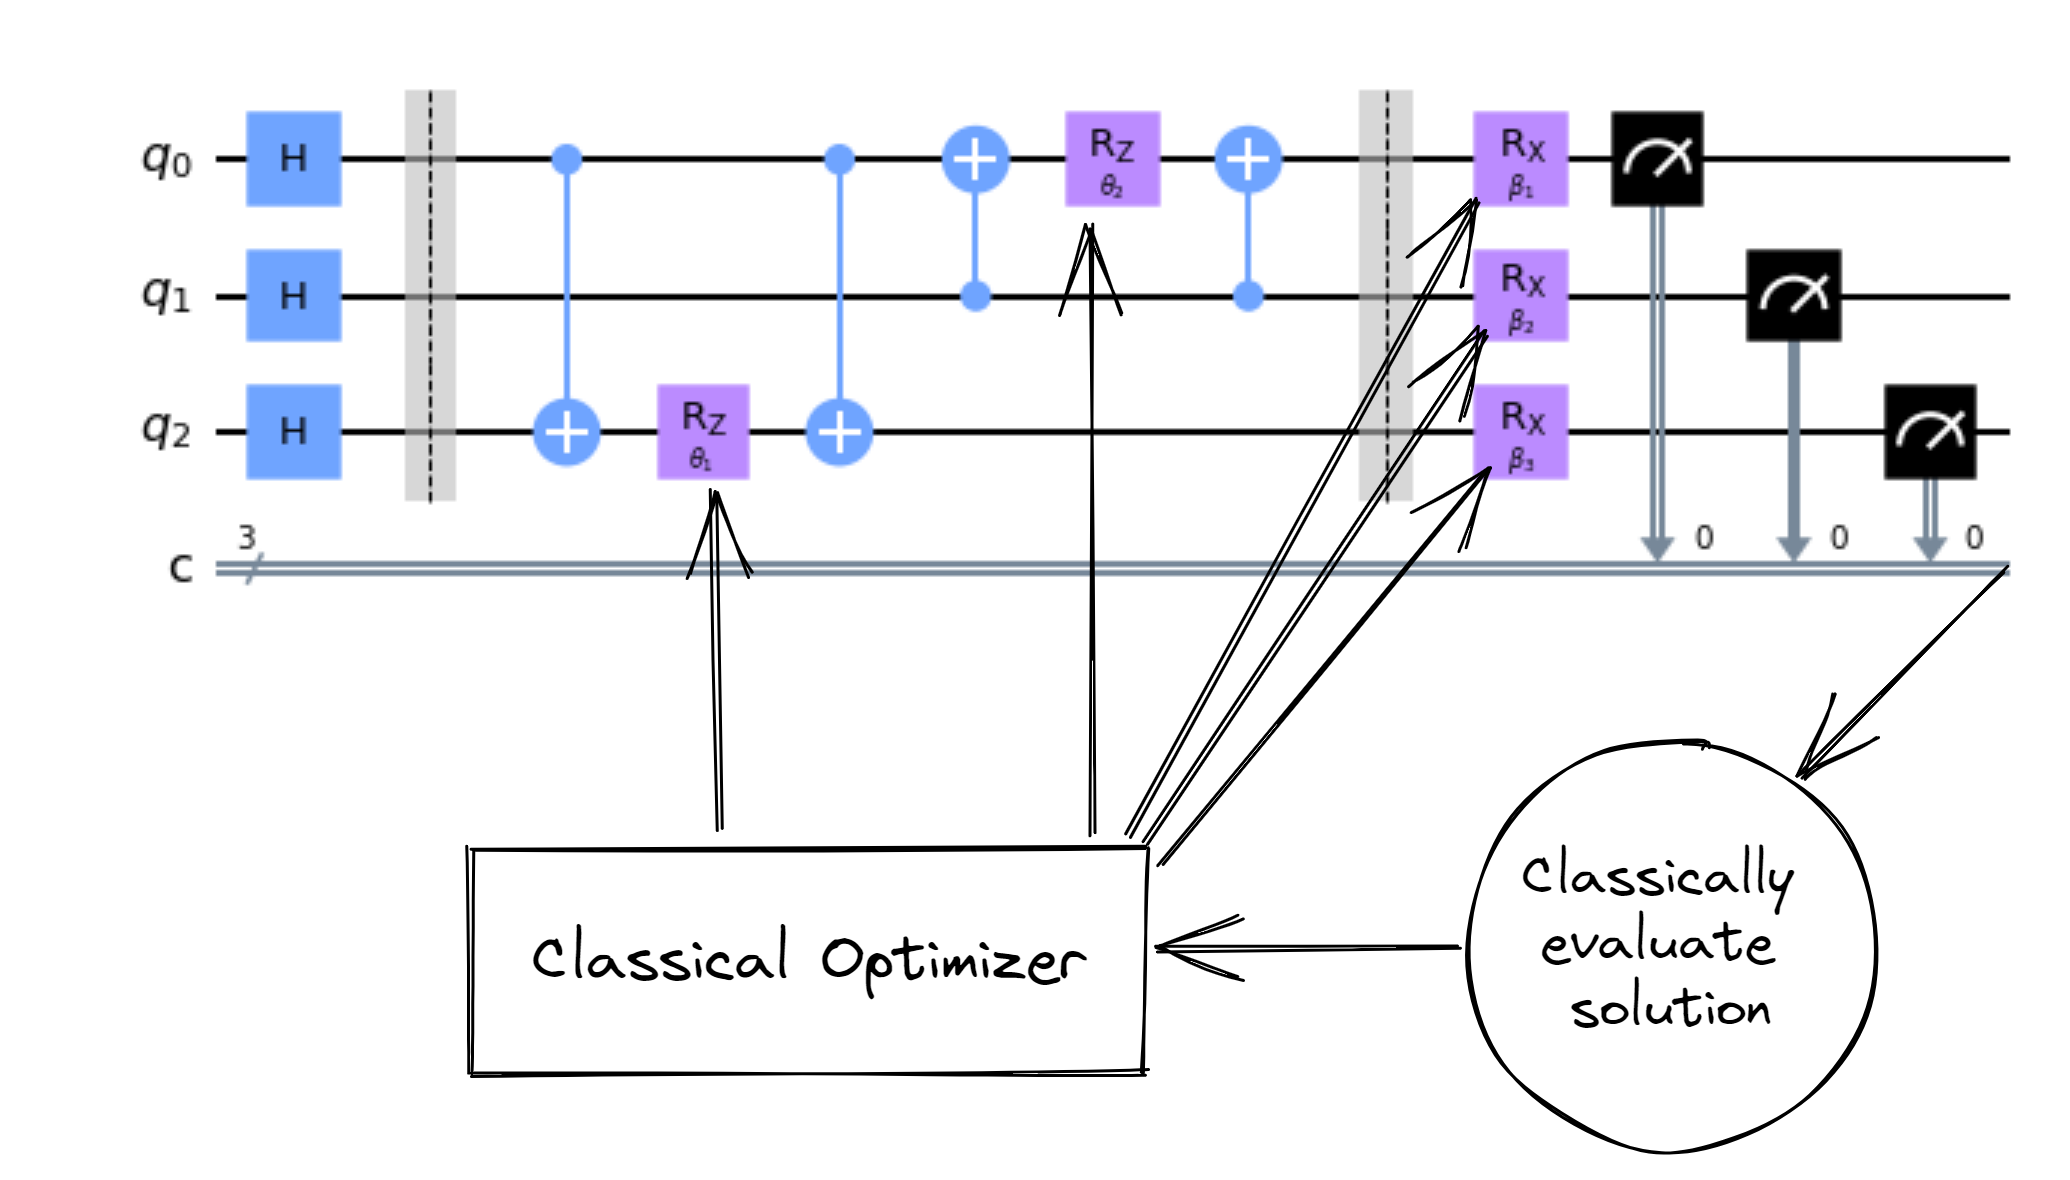
\includegraphics[width=0.7\linewidth]{figures/intro/qaoa-optimization.png}
    \caption[Variational Circuit for QAOA]{An example of a QAOA circuit with $p = 1$ blocks and generated to compute max-cut on a graph with 3-nodes and 2-edges between (0, 2) and (1, 0). The state generated by the circuit is parameterized in terms of the five parameters in the circuit. The output along the z-axis is measured and used to compute the classical loss value, i.e., the size of the max-cut given to which each node (represented by a qubit) belongs. Finally, a classical optimizer is used to reduce the value of the loss function such that resulting ansatz from the optimization process represents the cut of minimum size.}
\end{figure}

Quantum Approximate Optimization Algorithms are a class of variational quantum algorithms used as a general-purpose hammer to solve combinatorial optimization problems probabilistically \cite{qaoa-max-cut-farhi}.

\paragraph*{Motivation for the Algorithm}: The Algorithm takes inspiration from adiabatic quantum computing, which is a method that does the following: We start with a quantum state that is an easily preparable ground state of some Hamiltonian, and we vary this Hamiltonian sufficiently slowly and try to reach some target Hamiltonian, then the given quantum state will also track the ground state of the current form of the Hamiltonian. So the result of the Algorithm, if performed slowly enough, will be the ground state of the target Hamiltonian the preparation of which might not have been obvious otherwise.

QAOA takes that philosophy to the gate-computation model and uses the Suzuki-Trotter \cite{method-suzuki-trotter-decomposition} decomposition to approximate the application of unitaries corresponding to these Hamiltonians for sufficiently short periods of time.

\paragraph*{Algorithm}: The following steps are performed to execute QAOA for a given optimization problem.
\begin{enumerate}
    \item \textbf{Prepare the initial state}: We start by applying a Hadamard on all qubits to create an initial state which is an equal superposition of all basis states.
    \item \textbf{Apply the mixing unitary}: The mixing unitary corresponds to the mixing Hamiltonian as follows.
    \begin{equation}
        U(H_B) = e^{-i \beta H_B}
    \end{equation}
    We choose the mixer hamiltonian to be $X^{\otimes N}$, and the corresponding unitary becomes $R_x(\beta)^{\otimes N}$. This is because the ground state of this hamiltonian is known to be the initial state that we have prepared.
    \item \textbf{Apply the problem Hamiltonian}: The problem unitary corresponds to the Hamiltonian formulation of our problem, and this is the Hamiltonian for which we are attempting to find the ground eigenstate.
    \begin{equation}
        U(H_P) = e^{-i \gamma H_P}
    \end{equation}
    The hamiltonian needs to be formulated for each problem individually.
    \item \textbf{Repeat for p iterations}: We execute the mixing-Hamiltonian problem-Hamiltonian process for p-iterations. Each player is a $\beta$-duration mixing Hamiltonian and a $\gamma$-duration problem Hamiltonian application. For tuned values of $\beta$ and $\gamma$ and sufficiently large $p$, this can be made to approximate adiabatic computing.
    \item \textbf{Measure and classically compute loss}: The loss value that we are attempting to optimize is the following:
    \begin{equation}\label{eqn:loss-qaoa-circuit}
        \mathcal{L} = \braket{\psi(\beta, \gamma) \vert H_p \vert \psi(\beta, \gamma)}
    \end{equation}
    To compute this, we measure all qubits, and using the bitstring obtained in our classical registers, we classically compute the value of the optimization metric for this bitstring solution.
    \item \textbf{Classically compute derivatives and update parameters}: The parameters for each of the $p$ layers $(\beta, \gamma)$ are optimized using some method like gradient descent or adam. We attempt to reduce the value of the loss, as defined by the parameter updates in equation \ref{eqn:loss-qaoa-circuit}.
\end{enumerate}

\paragraph*{QAOA for Max Cut of a Graph}: Given a graph with vertices $v \in V$ and edges $e \in E \subset V \times V$, we want to compute a partition of vertices into two sets $f: V \rightarrow \{-1, +1\}$ such that the number of edges going across the partition ($C = \{ e = (u, v) | e \in E \;;\; f(u) \neq f(v) \}$) is maximized ($\max_{f} |C|$).

The QAOA formulation follows naturally. The classical loss function is the following:
\begin{equation}
    \mathcal{L} = \frac{-1}{2} \sum_{e = (u, v) \in E} (f(u) \cdot f(v) - 1)
\end{equation}
Since the Pauli-Z operator on the $\ket{0}$ and $\ket{1}$ state acts similar to the function $f$, in the quantum phrasing we can equivalently use the Z operators. We can drop the global constants and additive terms when writing out the optimization objective.
\begin{equation}
    \mathcal{H} = \frac{-1}{2} \sum_{e = (u, v)} I_0 \otimes I_1 \otimes \ldots \otimes Z_u \otimes \ldots \otimes Z_u \otimes \ldots \otimes I_N
\end{equation}
This can be efficiently implemented in a circuit, which will be used as the problem unitary.

\paragraph*{Other applications}: The QAOA algorithm can be further used to solve approximately other problems, including those that are NP-complete such as Weighted Max-Cut, 3-SAT, Travelling Salesman problem, amongst others. On the problem of Max-Cut, QAOA had, for a short span of about 3-months, held the best approximation ratio (\cite{qaoa-max-cut-farhi}) until it was superseded by semi-definite programming. Even though QAOA may not be able to be within the bounds achievable by classical computers, the universality of its applicability is remarkable. Coming up with classical methods to outperform QAOA on every new task takes much effort, semi-definite programming solutions have proven to be the best bet to outperform QAOA, but they have to be formulated afresh for each problem. Therefore, as a general-purpose solution to many problems, QAOA stands as a very good bet.


\subsection{Variational Quantum Eigensolvers}

Variational Quantum Algorithms is another entry in the class of variation algorithms, which tries to estimate the ground eigenstate and eigenvalues of a Hamiltonian using the method of optimization described above.

\begin{equation}
    \lambda_{min} \leq \braket{H}_{\psi} = \braket{\psi \vert H \vert \psi} = \sum_{i=1}^{N} \lambda_i \vert \braket{\psi_i \vert \psi} \vert ^2
\end{equation}

\section{Reinforcement Learning}

\subsection{What is Reinforcement Learning}

Machine Learning and all associated sub-disciplines are motivated by the goal of achieving artificial general intelligence, that is, being able to mimic the human mind and even surpass its capacity to perceive, compute and actuate. The human mind deals with various problems differing greatly in their phrasing, the solutions they admit, etc. This host of problem types requires many different types of learning methods in various settings.

Deep Learning is an extremely powerful and popular one of these methods, which uses parameterized function approximators (aka. neural networks) to learn arbitrary functions directly from examples. We typically learn functions that take as input numerical data and associated structure (e.g., graphs) and produce one or many continuous-valued outputs (regression) or discrete-value outputs (classification). This has been employed with great success in tasks like image recognition, text generation, etc.

Despite all their predictive power, these methods are limited in the problems they can solve. One limitation is our inability to provide many labeled examples since running laboratory experiments or expensive in-silico simulations are often too time and resource-consuming. Another issue is that the output may not be a simple function of its inputs. For instance, when predicting a compilation output to take at each step, our action chosen depends greatly on other actions scheduled, and therefore a single step function cannot solve such a problem; an iterative approach to optimize these coordinates is required. In such cases where a problem is solved in many steps, there is no notion of the correct result after a single step; we can only score if the composite of steps produces the final result. All these problems necessitate a machine learning method that can produce outputs over several timesteps and be able to reason about the correctness of its outputs based on rewards it may obtain at a different time in our process. This method is Reinforcement Learning. \cite{rl-intro-sutton-barto}


\subsubsection{Markov Decision Processes}

A Markov Decision process is any real or simulated process going on in time where each decision follows the Markovian Property, i.e., any future state transitions or rewards are conditionally independent of the past states and actions given the present state the environment is in.

A Markov Decision Process (MDP) can be represented as a tuple $\braket{S, A, T_a(s, s^\prime), R_a(s, s^\prime)}$, where $S$ is the set of all states, $A$ is the set of all actions available from any given state, $T_a(s, s^\prime)$ is the transition model which represents the probability of going from a starting state $s$ to a next state $s^\prime$ given that the action $a$ was taken, and $R_a(s s^\prime)$ is the reward obtained when this transition is realized.

Reinforcement Learning is a method of solving Markov Decision Processes. For our problem to be solved by RL, we need to ensure that our formulation is Markovian, i.e., our state has enough information to, given the action, predict the probability of the next state and the associated reward.

\subsubsection{Value Function and Policy Function}

At every point in time, our agent has access to the state and gets to choose an action. For this action, it receives a reward, and the state of the simulation is updated. 
This process continues indefinitely until a terminal state is reached, i.e., one where no further progress needs to be made and no future rewards can be collected. This entire trajectory of states and actions together comprises an episode.

The agent maintains a function which is called its \textbf{policy function} $\pi(s, a)$, which given the current state, gives the probability of each action it can take from that state. Our agent is allowed to be stochastic for various practical and theoretical reasons, so the probability for more than one action in a given state is allowed to be non-zero. This is the function that we shall attempt to optimize while learning from our environment.

While acting according to any policy function, we can associate each state with what we call the \textbf{value function} $V_{\pi}(s)$, which represents the expected sum of rewards till the end of the episode obtainable by following the policy. The optimal policy function $\pi$ leads to the maximum value function for the starting state.

Value-function of one state can be written in terms of that of others. To compute these values over all the states, we need to apply our updates iteratively.

\begin{equation}
    V(s) = \sum_{a \in A} \pi(s, a) \sum_{s^\prime} T_a(s, s^\prime) (V(s^\prime) + R_a(s, s^\prime))
\end{equation}

Instead of associating a value with each state, we can associate it with a state-action pair. This function is called the Q-function, and it carries equivalent information to the value function.
\begin{eqnarray}
    Q(s, a) &=& \sum_{s^\prime} T_a(s, s^\prime) \bigg(R(s, s^\prime) + V(s^\prime) \bigg)\\
            &=& \sum_{s^\prime} T_a(s, s^\prime) \bigg(R(s, s^\prime) + \sum_{a \in A} \pi(s^\prime, a) Q(s^\prime, a)\bigg)
            \label{eqn:defn-q-v-fn}
\end{eqnarray}

\subsection{Reinforcement Learning Algorithms}

In the following sections, we shall see three kinds of models:
\begin{itemize}
    \item Value Function Optimizers
    \item Policy Function Optimizers
    \item Actor-Critic Systems
    \item Planning based Reinforcement Learning
\end{itemize}


\subsubsection{Deep Q-Networks}

The first class of models attempts to approximate the value function. Assuming that our policy function will be that which is optimal, and assuming that our actions are deterministic (i.e., transition probabilities are 1 for the state we result in after an action and 0 otherwise), we can rewrite equation \ref{eqn:defn-q-v-fn} as:
\begin{eqnarray}\label{eqn:defn-q-fn}
    Q(s, a) \leftarrow R(s, s^\prime) + \max_{a \in A} Q(s^\prime, a)
\end{eqnarray}

For almost all problems in the real world, the state space is too large to maintain explicitly. Therefore we use a parameterized function $Q_{\theta}$, typically a neural network, to approximate the q-value from any given state-action pair.

The parameters $\theta$ can be updating using gradient based methods. The update operation is shown in equation \ref{eqn:q-update}.
\begin{equation}
    \label{eqn:q-update}
    \begin{split}
        \theta_{k+1} = \theta_k - \alpha \nabla_\theta \Bigg[\frac{1}{2} \bigg(Q_\theta(s, a) - \Big(R(s, a, s^\prime) + \gamma \max_{a^\prime} Q_{\theta_k}(s^\prime, a^\prime)  \Big) \bigg) \Bigg] \Bigg\vert_{\theta_k}
    \end{split}
\end{equation}

Several improvements to the training efficiency and stability of the DQN algorithm have been made; a few examples are the Double DQN by \cite{double-dqn}. This set of improvements put together has been analyzed by \cite{rainbow-dqn} under the name Rainbow DQN.

\subsubsection{Policy Function Approximators}

The policy function $\pi_\theta(s, a)$ gives the probability of each action given the state. In value function methods, we computed the policy by finding the action with the maximum expected value and assigning it a probability of 1 and other actions 0 for each state. When learning the policy directly, we use a stochastic policy instead, which chooses smooth and optimizable actions.

\paragraph{Reasons to use policy gradients:}

Following are the benefits of attempting to learn the policy directly instead of attempting to learn the value function and the policy through it:
\begin{enumerate}
    \item Learning value function may be much harder than learning the relative quality of actions. E.g., when compiling a circuit, it is tough to ascertain the value function of the state, which would correspond to the number of timesteps it would take to compile the remainder of the circuit; it's much easier to decide what action would best help make progress in the circuit compilation task. 
    \item We might want to obtain an inherently stochastic policy, where policy-based methods are the better choice. This often happens when we want to sample different action choices from our algorithm and rank them later.
    \item Many a time, the action space is continuous or intractably large, and maximizing the value over all the actions is not feasible. Here we can only use policy-based methods. The routing problem's action space fits the bill for this.
\end{enumerate}

\paragraph{Method:}
To optimize our policy, we sample trajectories from our policy and increase the probability of actions in trajectories that obtain high rewards and lower the probability of those with lesser rewards.

The utility of our policy is the expected reward under trajectories sampled from this policy; this is the quantity we wish to maximize over the parameters $\theta$. To perform this maximization, we compute $\nabla_\theta U(\theta)$ and update the parameter vector as $\theta \leftarrow \theta + \epsilon \nabla_\theta U(\theta)$. The gradient only depends on the gradient of the log of our policy function scaled by the rewards obtained along the trajectory and, very importantly, does not depend on the true transition model. Equation \ref{eqn:policy-grad} follows from a mathematically involved derivation done in \cite{policy-grad-theorem}.

\begin{equation}\label{eqn:policy-grad}
    \nabla_\theta U(\theta) \leftarrow \frac{1}{m} \sum_{i=1}^{m} \sum_{t=0}^{H-1} \nabla_\theta \log \pi_\theta (u_t^{(i)}|s_t^{(i)}) \Bigg(\sum_{k=t}^{H-1} R(s_k^{(i)}, u_k^{(i)}) - b(s_t^{(i)})\Bigg)
\end{equation}

\paragraph{Other Nuances:} Despite having the gradient that we need to update along, it is unclear what learning rate we should use to perform the said update. Unlike in deep learning, where the next iteration would correct if we overstep along the gradient, an overstep in our policy can lead to evaluation over an incorrect policy and can essentially wipe out all we have learned till now. Trust Region policy optimizations (TRPO) by \cite{trpo} and Proximal Policy Optimizations (PPO) by \cite{ppo} are methods that address this. Furthermore, to increase sample efficiency, Direct Deterministic Policy Gradients (DDPG) by \cite{ddpg}, and Soft Actor critic (SAC) \cite{sac} are used.

\subsubsection{Actor Critic Methods}

In equation \ref{eqn:policy-grad}, we are free to subtract a baseline value $b(s_t^{(i)})$ from the summed up rewards for each action; however, this baseline should be independent of the action and can only depend on the state. Subtraction of this baseline leads to lower variance estimates in the value of actions. The network now has to predict a quantity called the advantage. Advantage represents the difference in the value of each action over or below the expected reward obtainable from the state.
\begin{equation}\label{eqn:advantage}
    A(s, a) = Q(s, a) - V(s)
\end{equation}

This is implemented in practice using two networks, an actor network, which estimates the values of the actions, and a critic network, which estimates the resultant values of the states, which we subtract as a baseline from the rewards. These methods are often known to be stabler than their pure policy-gradient counterparts.

There are several variants on how the critic network and the explicit rollout together lead to the estimate of the value for each state, which has been discussed in detail by \cite{actor-critic-a2c, actor-critic-a3c, actor-critic-gae}

\subsubsection{Monte Carlo Tree Search}

When the transition model (next state and reward given action) is known, we can plan explicitly using a tree search. Since the tree would grow combinatorially big, we use reinforcement learning to find the most promising nodes. Monte Carlo Tree Search is one such method, which has gained prominence due to its use in AlphaGo by \cite{mcts-alphago} to play Go and in AlphaZero by \cite{mcts-alphazero} to play Chess, Go, and other games with no human supervision during training. 

The use of MCTS for Qubit Routing is discussed in much greater detail in the following chapter.